% !TeX root = ../libro.tex
% !TeX encoding = utf8

%\setchapterpreamble[c][0.75\linewidth]{%
%	\sffamily
%  Breve resumen del capítulo. TODO
%	\par\bigskip
%}

\chapter{Códigos convolucionales}\label{ch:cuarto-capitulo}

En este capítulo vamos a estudiar una clase de códigos muy distintos a los códigos de bloque vistos en el capítulo anterior, llamados \emph{códigos convolucionales}. Recordemos que el propósito de los códigos es codificar la información de manera que se puedan \emph{corregir los errores} que se han producido en la transmisión. La información que se suele enviar es demasiado larga como para ser procesada de una única vez, por tanto, esta información se divide en varios bloques, y en el caso de los códigos de bloque, se procesan de manera independiente.

\begin{figure}[h]
    \centering
    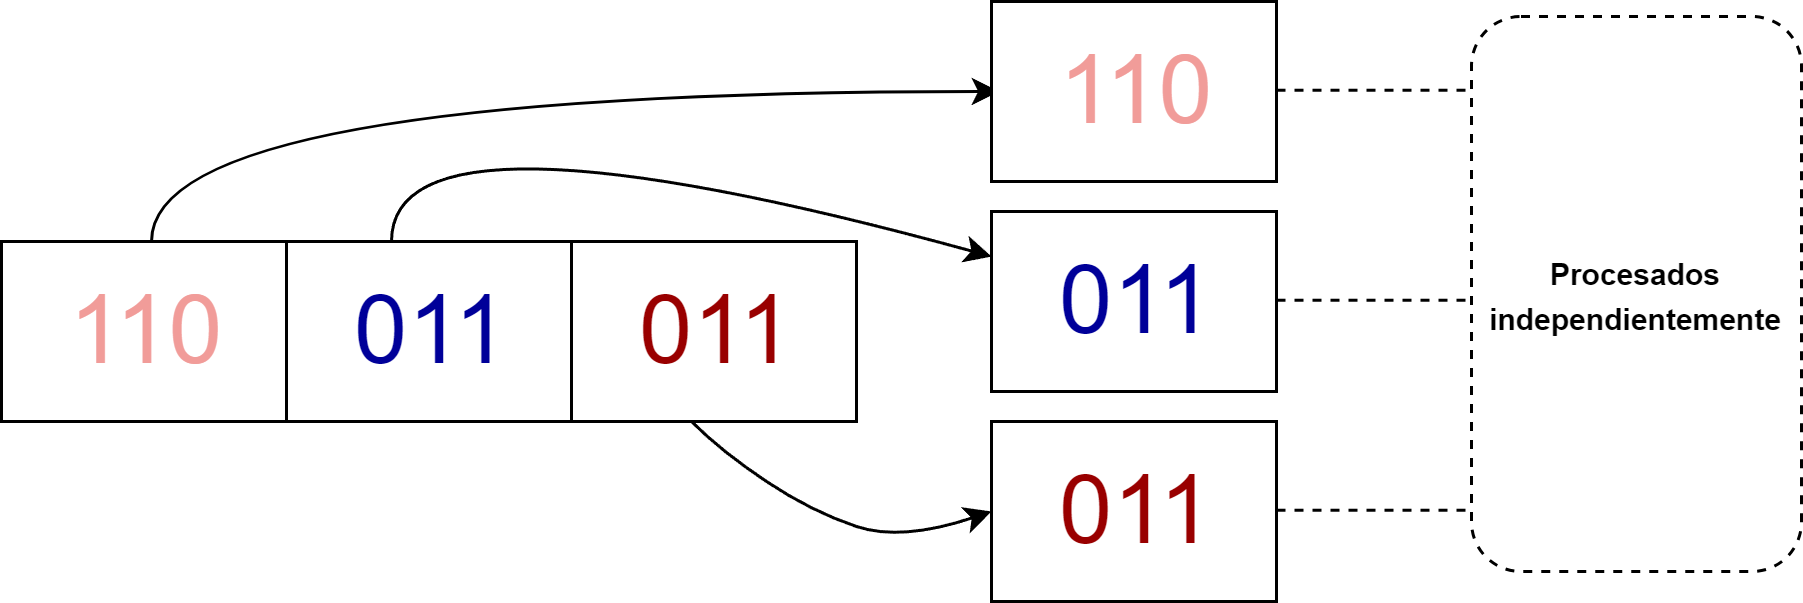
\includegraphics[width=0.7\textwidth]{img/codbloque.png}
    \caption{Funcionamiento códigos de bloque.}
    \label{fig:codbloque}
\end{figure}

Por otro lado, los códigos convolucionales utilizan un esquema de codificación que no depende únicamente del mensaje actual que se está transmitiendo, sino también de un cierto número de mensajes anteriores. Así, podríamos decir que, a diferencia de los códigos de bloque, un codificador de un código convolucional tiene "memoria".

\begin{figure}[h]
    \centering
    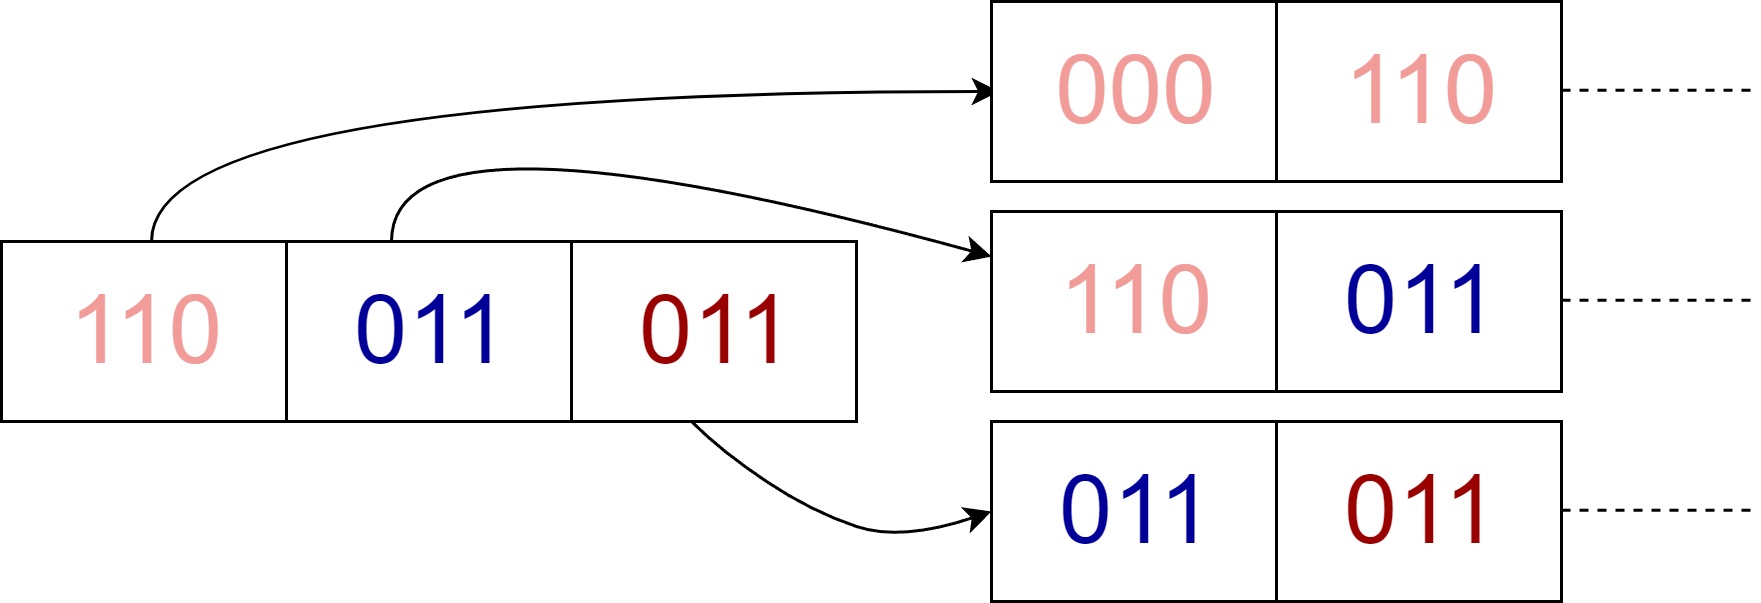
\includegraphics[width=0.7\textwidth]{img/codconvolucionales.png}
    \caption{Funcionamiento códigos convolucionales.}
    \label{fig:codconvolucional}
\end{figure}

Los códigos convolucionales fueron presentados por primera vez por Peter Elias  \cite{Elias1955} en 1955 como una alternativa a los códigos de bloque. El primer algoritmo de decodificación para estos códigos fue la decodificación secuencial sugerida por Wozencraft \cite{Wozencraft1957SequentialDF} en 1957 y posteriormente desarrollada por Fano, quien en 1963 propuso un método de decodificación muy ingenioso \cite{Fano1963}. Se desarrollaron muchos más algoritmos de decodificación para estos códigos, pero sin duda, el algoritmo de decodificación principal para estos códigos es el \emph{algoritmo de Viterbi}, el cual es un algoritmo de programación dinámica desarrollado por el ingeniero italiano A.J Viterbi \cite{Viterbi1967} en 1967.

Si bien estos códigos se desarrollaron en los años 50, no fue hasta 1970 cuando Forney \cite{Forney1970} desarrolló por primera vez una teoría algebraica sólida. No obstante, la teoría matemática existente para los códigos convolucionales no está tan desarrollada como lo está para los códigos de bloque. A lo largo de este capítulo presentaremos de varias formas los códigos convolucionales y estudiaremos cómo podemos codificar estos códigos mediante matrices generadoras.

Las principales fuentes para la redacción de este capítulo han sido \cite{Huffman_Pless_2010}, \cite{Forney1970}, \cite{Johannesson2015} , \cite{cccheide} y \cite{jl2020}.


\section{Matrices generadoras y codificación de códigos convolucionales}

Existen numerosas formas de definir los códigos convolucionales como veremos a lo largo del trabajo. Usualmente, los códigos convolucionales se han estudiado principalmente para el cuerpo $\F _2$, sin embargo, en los últimos años se han estudiado en ámbitos más generales, donde $\F$ es un cuerpo finito arbitrario.

Sea $\F$ un cuerpo finito y sea $t$\footnote{El símbolo $t$ representa el operador delay en los códigos convolucionales. En otras referencias bibliográficas (ver por ejemplo \cite{Huffman_Pless_2010}) se denota por $D$. } una indeterminada. Entonces, $\F[t]$ es el conjunto de todos los polinomios en la variable $t$ con coeficientes en $\F$. Este conjunto es un \emph{dominio de integridad} y, por tanto, podemos construir su \emph{cuerpo de fracciones}, al cual denotaremos $\F(t)$.

\begin{definicion}
    Un \emph{$(n,k)$-código convolucional} $\C$ es un subespacio $k$-dimensional de $\F(t)^n$.
\end{definicion}

Nótese que al ser $\F(t)$ un cuerpo infinito, $\C$ contendrá un número infinito de palabras código.

\begin{definicion}
    Sea $\C$ un $(n,k)$-código convolucional. El \emph{ratio} $R$ de $\C$ se define como $R = \frac{k}{n}$.
\end{definicion}

A diferencia de lo que ocurría con los códigos de bloque, no es usual considerar valores de $n$ y $k$ altos. Esto se debe a que la decodificación de códigos convolucionales es mucho más compleja.

\begin{definicion}
    Se dice que $G(t) \in \mathcal{M}_{k \times n}(\F(t))$ es una \emph{matriz generadora} de $\C$ si sus filas forman una base de $\C$.
\end{definicion}

Si $G(t)$ es una matriz generadora, entonces también lo será cualquier matriz obtenida como el producto de $G(t)$ y un elemento no nulo de $\F(t)$. Por tanto, si multiplicamos $G(t)$ por el mínimo común múltiplo de los denominadores de todas las entradas de la matriz, obtendremos una matriz generadora de $\C$ cuyas entradas están formadas por polinomios. Por tanto, cualquier código convolucional tiene una matriz generadora cuyas entradas son polinómicas. Dichas matrices reciben el nombre de \emph{matrices generadoras polinómicas} para $\C$.

\begin{ejemplo}
Sea $G_1(t) = \left[1 + t^2 \ \ \frac{1}{1 + t}\right]$ una matriz generadora de un $(2,1)$-código convolucional binario. Entonces la matriz $G_2(t) = (1+t)G_1(t) = \left[1 + t + t^2 + t^3 \ \ \ 1  \right]$ es una matriz generadora polinómica de $\C$.
\end{ejemplo}


Utilizaremos estas matrices para codificar mensajes. Partiremos de la suposición de que estos mensajes son \emph{finitos} \footnote{En teoría de códigos convolucionales es común trabajar con mensajes de longitud infinita, los cuales pueden representarse mediante series de Laurent formales en el cuerpo $\F((t)).$} y los representaremos mediante polinomios $x(t) = \sum_{i=0}^{L-1} x(i)t^i \in \F[t]^k$.

Vamos a describir el procedimiento de codificación para un $(n,k)$-código convolucional $\C$ utilizando una matriz generadora polinómica $G(t)$. Para enfatizar la conexión entre $G(t)$ y el proceso de codificación, a menudo nos referiremos a $G(t)$ como \emph{codificador}. Empezaremos suponiendo que $k = 1$, de esta manera, en cada momento $i = 0,1,\dots$ la entrada para el codificador $G(t)$ está formada por un único elemento $x(i) \in \F$. 

Supongamos que tenemos un flujo de entrada de $L$ elementos, cada uno de estos pertenecientes a $\F$. Estos elementos se representan como coeficientes de un polinomio $x(t)$, donde $t$ es una indeterminada que representa el operador delay. El polinomio se define como $x(t) = \sum_{i=0}^{L-1}x(i)t^i$, donde $x(i)$ es el símbolo $i$ del flujo de entrada. La codificación, al igual que con los códigos de bloque, se realiza mediante el producto $x(t)G(t) = c(t)$. La palabra código $c(t) = (c_1(t),\dots,c_n(t))$ tiene $n$ componentes, los cuales son polinomios \footnote{ Si suponemos que el codificador $G(t)$ no es polinómico, entonces $c(t)$ puede ser un elemento del cuerpo de fracciones $\F(t)^n$. } en $t$.

\begin{ejemplo}
Sea $\C$ un $(2,1)$-código convolucional binario y sea $G(t) = \left[ 1 + t + t^2 \ \ 1 + t^2 \right]$ su matriz generadora. Vamos a codificar el mensaje $\mathbf{m} = 110101$, cuya longitud es $L = 6$. Este mensaje corresponde al polinomio $x(t) =  \sum_{i=0}^{5}x(i)t^i = 1 + t + t^3 + t^5$. Lo codificamos utilizando la matriz generadora $G(t)$:
\begin{align*}
    c(t) &= x(t)G(t) \\
    &= (1 + t + t^3 + t^5)\left[ \begin{array}{cc}
    1 + t + t^2 & 1 + t^2 \\
    \end{array} \right] \\
    &= \left(1 + t^4 + t^6 + t^7, \ 1 + t + t^2 + t^7\right) \\
    &= (c_1(t), c_2(t)).
\end{align*}
Si observamos detenidamente las multiplicaciones y las sumas realizadas para calcular $c_1(t)$ y $c_2(t)$, podemos ver que tanto la memoria como el operador delay $t$ \emph{juega un papel crucial}. Puesto que $c_1(t) = x(t)(1 + t + t^2)$, en el momento $i$, observamos que $c_1(i) = x(i)(1 + t + t^2) = x(i) + x(i-1) + x(i-2)$. De manera análoga, se tiene que $c_2(i) = x(i) + x(i-2)$, estas ecuaciones reciben el nombre de \emph{ecuaciones del codificador}. Cada aparición de $t^j$ retrasa la entrada en $j$ unidades de tiempo. Diremos que la memoria del codificador es $M = 2$.
\end{ejemplo}

\begin{definicion}
Sea $\C$ un $(n,k)$-código convolucional y sea $G(t) \in \mathcal{M}_{k \times n}(F[t])$ una matriz generadora polinómica de este código. Sean $g_{ij}(t)$ los elementos de $G(t)$. Se define la \emph{memoria $M$ de $G(t)$} como el mayor grado de cualquier elemento de $G(t)$, es decir,
$$ M = \max_{\substack{1 \leq i \leq k \\ 1 \leq j \leq n}} \left\{ \gr(g_{ij}(t)) \right\}.$$
\end{definicion}

Algo a tener en cuenta es que la memoria \emph{depende exclusivamente del codificador} $G(t)$ y no del código $\C$. Recordemos que si multiplicamos la matriz $G(t)$ por cualquier elemento no nulo de $\F[t]$, seguirá siendo una matriz generadora para $\C$, sin embargo, su memoria puede cambiar.

Podemos generalizar el proceso de codificación anterior a un $k$ arbitrario. En esta ocasión, la entrada en el instante $i = 0,1,\dots$ está formada por los elementos $x_j(i) \in \F, \ j \in \{1,\dots,k\}$, los cuales forman el mensaje $\mathbf{x}(i) = (x_1(i),\dots,x_k(i))$. Al igual que antes, podemos reescribir cada $x_j$ como un polinomio en la indeterminada $t$. De esta forma, la entrada resultante $\textbf{x}(t)$ será un vector de $k$ polinomios. La palabra código se calcula, de nuevo, como $\mathbf{x}(t)G(t) = \mathbf{c}(t) = (c_1(t),c_2(t),\cdots,c_n(t))$. Veamos un ejemplo.

\begin{ejemplo}
Sea $\C$ un $(4,2)$-código convolucional binario y sea $$G(t) = \left[ \begin{array}{cccc}
    1 & 1 + t + t^2 & 1 + t^2 & 1 + t \\
    0 & 1 + t & t & 1 \\
    \end{array} \right]$$ 
una matriz generadora. Vamos a codificar el mensaje $\mathbf{m} = (11010,10111)$, el cual corresponde al par polinómico $\mathbf{x}(t) = (1 + t + t^3,1 + t^2 + t^3 + t^4)$. Lo codificamos mediante la matriz generadora $G(t)$:

\begin{align*}
    \mathbf{x}(t)G(t) &= (1 + t + t^3, 1 + t^2 + t^3 + t^4) \left[ \begin{array}{cccc}
        1 & 1 + t + t^2 & 1 + t^2 & 1 + t \\
        0 & 1 + t & t & 1 \\
    \end{array} \right] \\
    &= (1 + t + t^3, 1 + t^2 + t^4, 1 + t^2 + t^3 + t^4, 0 ) = \mathbf{c}(t).
    \end{align*}

Como el máximo grado de los elementos de $G(t)$ es $2$, sabemos que su memoria $M$ será también $2$. Podemos también calcular las ecuaciones del codificador $G(t)$ de manera análoga al caso $k=1$.

\[
\left\{
\begin{aligned}
    c_1(i) &= x_1(i), \\
    c_2(i) &= x_1(i) + x_1(i-1) + x_1(i-2) + x_2(i) + x_2(i-1),   \\
    c_3(i) &= x_1(i) + x_1(i-2) + x_2(i-1),\\
    c_4(i) &= x_1(i) + x_1(i-1) + x_2(i).\\
\end{aligned}
\right.
\]
\end{ejemplo}

Hemos visto como se puede codificar un mensaje mediante códigos convolucionales de forma matemática mediante la matriz generadora $G(t)$. Sin embargo, es interesante estudiar cómo podríamos construir un \emph{codificador físico} \footnote{Nos centraremos en el caso en el que el cuerpo es $\F_2$ pues, al tratarse de 1's y 0's, su implementación es más sencilla. } mediante registros de desplazamiento. Para codificar códigos convolucionales podemos usar registros de desplazamiento con retroalimentación lineal, un tipo particular de registros de desplazamiento en el que la entrada es un bit proveniente de aplicar una función de transformación lineal a un estado anterior. Los componentes principales de estos registros son los elementos de delay (también llamados flip-flops) y los sumadores binarios mostrados en la Figura \ref{fig:encoder}.

\begin{figure}[h]
    \centering
    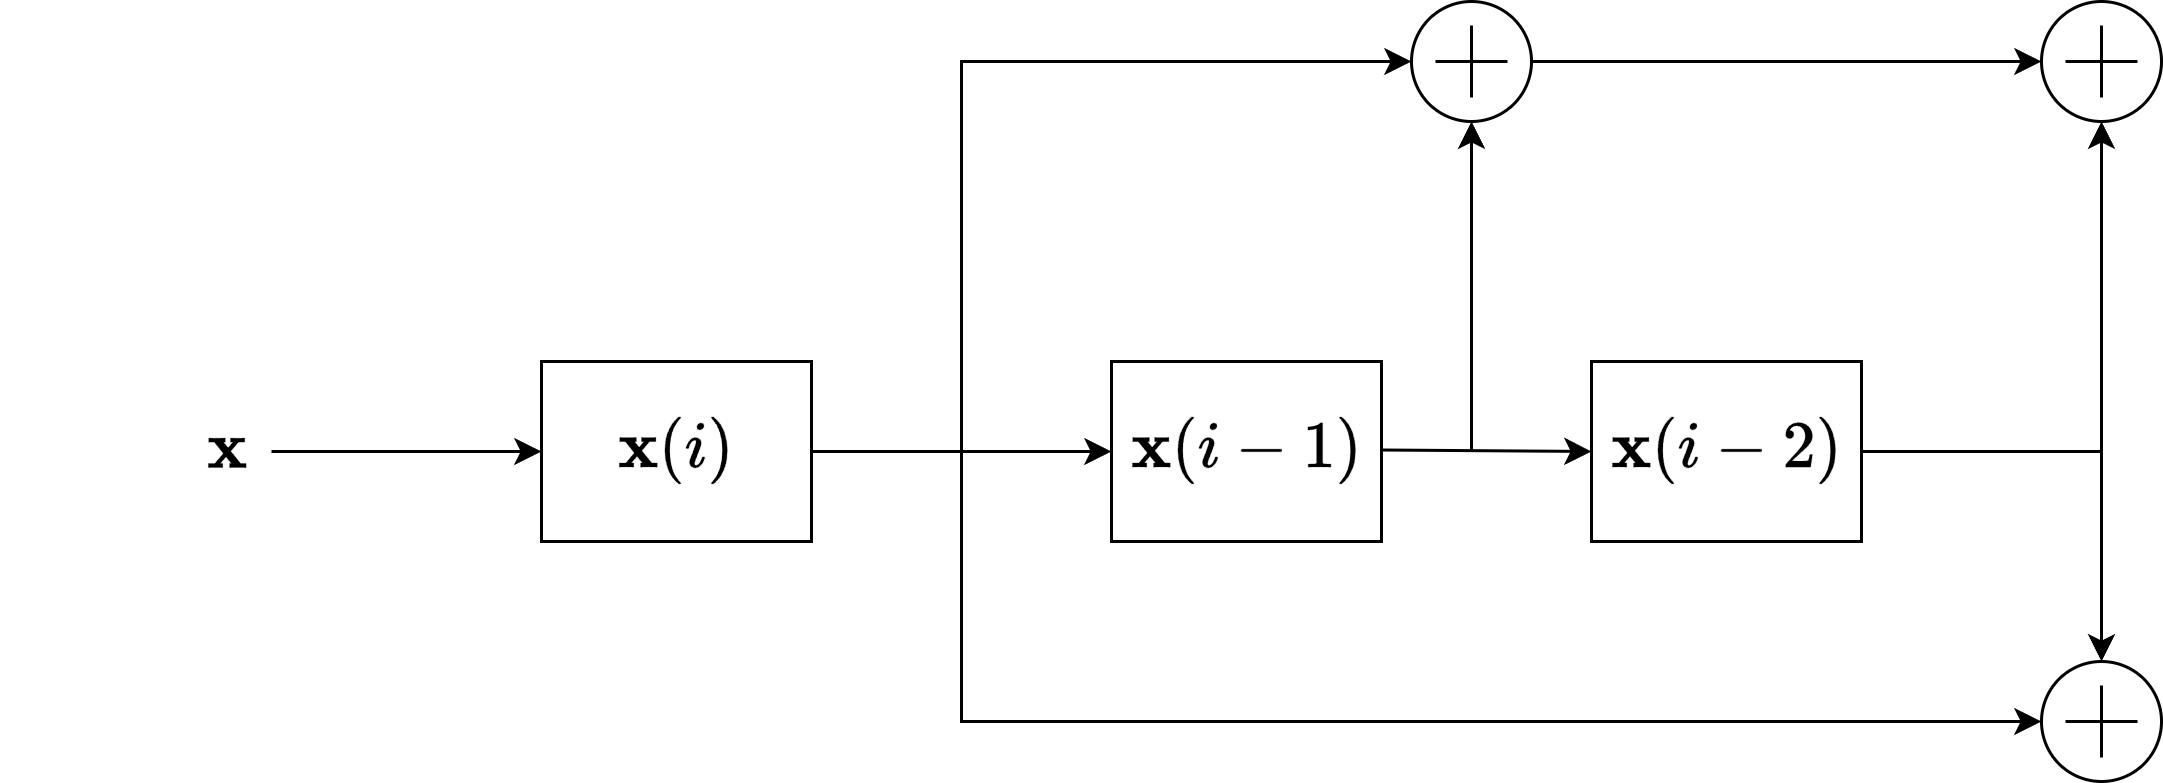
\includegraphics[width=0.8\textwidth]{img/codfisico.png}
    \caption{Codificador físico para $G(t) = \left[ 1 + t + t^2 \ \ 1 + t^2 \right]$.}
    \label{fig:encoder}
\end{figure}

\section{Matrices generadoras canónicas}

Hemos visto que un código convolucional $\C$ puede tener varias matrices generadoras, incluyendo matrices cuyas entradas son funciones racionales. Hasta ahora, nos hemos enfocado en las matrices generadoras polinómicas, pero en esta sección, definiremos una subclase de las matrices generadora polinómicas: las \emph{matrices generadoras canónicas}.


Empecemos con unas definiciones importantes. Sea $G(t) = [g_{ij}(t)]$ una matriz polinómica de dimensión $k\times n$.

\begin{definicion}
 Se define \emph{el grado $m_i$ de la $i$-ésima fila de $G(t)$}  como el máximo grado de cualquier elemento de la fila $i$, para $i \in \{1,\dots,k\}$. Es decir,
$$m_i = \max_{1 \leq j \leq n} \gr(g_{ij}(t)).$$
\end{definicion}

\begin{definicion}
Se define el \emph{grado externo} de $G(t)$, denotado extdeg($G(t)$), como la suma de los grados de las $k$ filas de $G(t)$. Es decir,
$$\extdeg(G(t)) = \sum_{i=1}^{k} m_i.$$
\end{definicion}

\begin{ejemplo}
\label{ej:cc}
Sea $G_1(t) = \left[1 + t + t^2 \ \ 1 \right]$ una matriz generadora de un $(2,1)$-código convolucional binario. Como solo tiene una fila, su grado externo y el grado de la fila $1$ coinciden, y este es $2$.


Sea $G_2(t) = \left[ \begin{array}{cccc}
    1 & 1 + t + t^2 & 1 + t^2 & 1 + t \\
    0 & 1 + t & t & 1 \\
\end{array} \right]$ una matriz generadora de un $(4,2)$-código convolucional binario. Entonces $m_1 = 2$, $m_2 = 1$ y, por tanto, extdeg($G(t)$) $ = m_1 + m_2 = 3$. 
\end{ejemplo}

\begin{definicion}
Una \emph{matriz generadora canónica} para un código convolucional $\C$ es una matriz generadora polinómica cuyo grado externo es el mínimo posible entre todas las posibles matrices generadoras polinómicas para $\C$.
\end{definicion}


Por definición, todos los códigos convolucionales cuentan con una matriz generadora canónica. Este grado externo mínimo recibe el nombre de \emph{grado} del código $\C$.

Nótese que la matriz generadora canónica no es única (salvo el caso en el que el cuerpo sea $\F_2$), ya que podemos multiplicar esta matriz por cualquier elemento de $\F$ y seguiría conservando el grado externo.

\begin{ejemplo}
\label{ej:mgc}
Vamos a demostrar que la matriz generadora $G_1(t)$ del ejemplo \ref{ej:cc} es canónica para el $(2,1)$-código convolucional binario $\C$. En este caso, el grado externo de cualquier matriz generadora polinómica de $\C$ es el grado máximo de sus entradas (pues solo tiene una fila). Cualquier otra matriz generadora $G_1'(t)$ de $\C$ puede obtenerse de $G_1(t)$ multiplicando esta por un elemento de $\F(t)$, es decir, por una expresión del tipo $p(t)/q(t)$, donde $p(t),q(t) \in \F[t]$ (con $q(t) \neq 0$). Supondremos que $p(t)$ y $q(t)$ son polinomios coprimos (en caso contrario solo habría que simplificar). De esta forma, $G_1'(t) = \frac{p(t)}{q(t)}G_1(t)$. 

Como las matrices generadoras canónicas son polinómicas, $q(t)$ debe dividir a los dos elementos de $G_1(t)$ y como el segundo elemento es $1$, $q(t) = 1$. Por tanto, $G_1'(t) = p(t)G_1(t)$. De esta manera, para que no aumente el grado debe ocurrir que $\gr(p(t)) = 0$, o lo que es lo mismo, $p(t) \in \F$. Esto demuestra que $G_1(t)$ es una matriz generadora canónica.
\end{ejemplo}

El razonamiento del Ejemplo \ref{ej:mgc} nos dice que si $\C$ es un $(n,1)$-código convolucional, una matriz generadora polinómica $G(t)$ será canónica si y solo si el máximo común divisor de sus entradas es $1$. Esto no es tan fácil cuando $k > 1$. A lo largo de esta sección buscaremos una condición \emph{necesaria y suficiente} para que una matriz generadora polinómica sea una matriz generadora canónica de un $(n,k)$-código convolucional. Antes de demostrarlo vamos a introducir los siguientes conceptos.

\begin{definicion}\label{def:complejidad}
Sea $G(t)$ una matriz polinómica de dimensión $k\times n$, con $k \leq n$. El \emph{grado interno} de $G(t)$, denotado como intdeg($G(t)$), es el máximo grado de todos los menores \footnote{Un menor de dimensión $k \times k$ de una matriz $M$ de dimensión $k \times n$, $k \leq n$ es el determinante de una matriz formada por $k$ columnas de $M$. La matriz $M$ tiene $\binom{n}{k}$ menores.} de $G(t)$ de dimensión $k \times k$. También se suele llamar \emph{complejidad del código}. Un código de complejidad $0$ es un código de bloque.
\end{definicion}

\begin{definicion}
Se dice que una matriz generadora polinómica de un código convolucional $\C$ es \emph{básica} si su grado interno es mínimo.
\end{definicion}

\begin{definicion}
Una matriz polinómica $G(t)$ es \emph{reducida} si entre todas las matrices de la forma $U(t)G(t)$, donde $U(t)$ es una matriz unimodular \footnote{Una matriz $U$ de dimensión $k \times k$ es \emph{unimodular} si su determinante es $1$.} de dimensión $k \times k$, $G(t)$ tiene el grado externo más pequeño.
\end{definicion}

En \cite{mceliece1998}, McEliece dio seis formulaciones equivalentes para que una matriz sea básica y tres para que sea reducida. Presentaremos algunas de estas equivalencias y omitiremos las demostraciones. Estas pueden ser encontradas en \cite[Apéndice A]{mceliece1998}.

\begin{teorema}
\label{th:cc1}
Sea $G$ una matriz generadora polinómica de un $(n,k)$-código convolucional. Equivalen las siguientes afirmaciones:
\begin{itemize}
    \item[(i)] La matriz $G$ es básica.
    \item[(ii)] El máximo común divisor de los menores $k \times k$ de $G(t)$ es $1$.
    \item[(iii)] Existe una matriz $K(t) \in \mathcal{M}_{n \times k}(\F[t])$ tal que $G(t)K(t) = I_k$.
    \item[(iv)] Si $\mathbf{c}(t) \in \F[t]^n$ y $\mathbf{c}(t) = \mathbf{x}(t)G(t)$, entonces $\mathbf{x}(t) \in \F[t]^k$.
\end{itemize}
\end{teorema}

Recordemos que la matriz $K(t)$ en (iii) es la inversa por la derecha de $G(t)$. La equivalencia (iii) del Teorema \ref{th:cc1} establece que si $G(t)$ es un codificador básico, entonces siempre que la entrada sea polinomial, también lo será la salida. La prueba de que (iii) implica (iv) es simple. Si (iii) se verifica y $\mathbf{c}(t) = \mathbf{x}(t)G(t)$, entonces $\mathbf{x}(t) = \mathbf{x}(t)I_k = \mathbf{x}(t)G(t)K(t) = \mathbf{c}(t)K(t)$. Como $c(t)$ y $K(t)$ solo tienen entradas polinomiales, también las tendrá $\mathbf{x}(t)$.

\begin{definicion}
El \emph{grado} de un vector $\mathbf{v}(t) \in \F[t]^n$ es el mayor grado de cualquiera de sus componentes. \footnote{Nótese que esta definición es consistente con la definción que hemos dado antes del grado de una matriz.}
\end{definicion}

\begin{teorema}
\label{th:aux}
Sea $G(t) \in \mathcal{M}_{k \times n}(\F[t])$ y sea $g_i(t)$ la i-ésima fila de $G(t)$. Equivalen las siguientes afirmaciones:
\begin{itemize}
    \item[(i)] La matriz $G$ es reducida.
    \item[(ii)] $\intdeg(G(t)) = \extdeg(G(t))$.
    \item[(iii)] Para cualquier $\mathbf{x}(t) = (x_1(t),\dots,x_k(t)) \in \F[t]^k$, se verifica 
    $$\gr(\mathbf{x}(t)G(t)) = \max_{i \leq i \leq k} \{\gr(x_i(t)) + \gr(g_i(t))\}.$$  
\end{itemize}
\end{teorema}

Nuestro objetivo será probar que una matriz generadora polinómica de un $(n,k)$-código convolucional es canónica si y solo si es básica y reducida. Para ello, necesitaremos el siguiente lema.

\begin{lema}
\label{lm:cc1}
Sea $G(t) \in \mathcal{M}_{k \times n}(\F[t])$ una matriz generadora polinómica de un código convolucional $\C$, $ k \leq n$. Sea $N(t)$ una matriz no singular de dimensión $k \times k$ con entradas en $\F[t]$. Se verifican las siguientes afirmaciones:
\begin{itemize}
    \item[(i)] $\intdeg(N(t)G(t)) = \intdeg(G(t)) + \deg(\det(N(t)))$.
    \item[(ii)] $\intdeg(G(t)) \leq \intdeg(N(t)G(t))$. La igualdad se verifica si y solo si $N$ es unimodular.
    \item[(iii)] $\intdeg(G(t)) \leq \extdeg(G(t))$.  
\end{itemize}
\end{lema}

\begin{proof}
Para probar (i) observamos que las submatrices de dimensión $k \times k$ de $N(t)G(t)$ son precisamente las submatrices $k \times k$ de $G(t)$ multiplicadas por $N(t)$ a la izquierda. Por tanto, los menores $k \times k$ de $N(t)G(t)$ son exactamente los menores $k \times k$ de $G(t)$ multiplicados cada uno por $\det(N(t))$. Lo que prueba (i). 

La parte (ii) se deduce de (i). 

Para (iii), supongamos que el grado de la $i$-ésima fila de $G(t)$ es $m_i$. Entonces, extdeg($G(t)$) $m_1 + \cdots + m_k$. Cualquier menor $k \times k$ de $G(t)$ es una suma de productos de entradas de $G(t)$, con un factor de cada fila en cada producto. Por tanto, el mayor grado posible del producto es  $m_1 + \cdots + m_k$, lo que prueba (iii).  
\end{proof}

Con este resultado, podemos probar el teorema principal de esta sección, el cual caracteriza las matrices canónicas de un código convolucional.

\begin{teorema}
Una matriz generadora polinómica de un $(n,k)$-código convolucional $\C$ es canónica si y solo si es básica y reducida.
\end{teorema}

\begin{proof} \phantom{}

\boxed{\Rightarrow}

Sea $G$ una matriz generadora canónica para $\C$. Sea $d_0$ el grado interno de las matrices generadoras básicas, que recordemos que es mínimo. Elegimos de entre todas las matrices generadoras básicas, una matriz $G_0(t)$ con grado externo mínimo.

Sea $U(t)$ una matriz unimodular de dimensión $k \times k$. Entonces utilizando el Lema \ref{lm:cc1}, $$U(t)G_0(t) = \intdeg(G_0(t)) = d_0.$$

Por definición de $G_0(t)$, $\extdeg(U(t)G_0(t)) \geq \extdeg(G_0(t))$ (ya que $U(t)G_0(t)$ genera $\C$), lo que implica que $G_0(t)$ es reducida. Teniendo en cuenta que $G_0(t)$ tiene el grado interno más pequeño de entre todas las matrices generadoras polinómicas de $\C$, $\intdeg(G_0(t)) \leq \intdeg(G(t))$. Pero intdeg($G(t)$) $\leq$ extdeg($G(t)$) por el Lema \ref{lm:cc1} y extdeg($G(t)$) $\leq$ extdeg($G_0$) por definición, ya que $G(t)$ es canónica. Por tanto,

\begin{equation}
\label{ec:1}
\intdeg(G_0(t)) \leq \intdeg(G(t)) \leq \extdeg(G(t)) \leq \extdeg(G_0(t)).
\end{equation}

Como $G_0(t)$ es reducida, $\intdeg(G_0(t)) = \extdeg(G_0(t))$ por el Teorema \ref{th:aux}. Y, por tanto, se da la igualdad en \eqref{ec:1}. 

De esta manera, $\intdeg(G(t)) = \intdeg(G_0(t)) = d_0$ probando que $G(t)$ tiene también grado interno mínimo entre todas las matrices generadoras polinómicas de $\C$, lo que implica que es básica. Como $\intdeg(G(t)) = \extdeg(G(t))$, obtenemos que $G(t)$ también es reducida.

\boxed{\Leftarrow}

Supongamos ahora que $G(t)$ es una matriz generadora polinómica de $\C$ reducida y básica. Sea $G_0(t)$ otra matriz generadora polinómica de $\C$. Por el Lema \ref{lm:cc1}, $\extdeg(G_0(t)) \geq \intdeg(G_0(t))$. Como $G(t)$ es básica, intdeg($G_0(t)$) $\geq$ intdeg($G(t)$). Y como también es reducida, $intdeg(G(t)) = \extdeg(G(t))$. Combinando estas desigualdades, llegamos a que extdeg($G_0(t)$) $\geq$ extdeg($G(t)$). Lo que implica que $G(t)$ es canónica, al ser $G_0(t)$ una matriz generadora polinómica arbitraria.
\end{proof}

\section{Códigos convolucionales y módulos}

Hasta ahora, hemos visto a los códigos convolucionales como subespacios $k$-dimensionales del cuerpo de fracciones $\F(t)^n$. Sin embargo, existen \emph{varias definiciones de códigos convolucionales} y algunos autores han utilizado la teoría de módulos para describir los códigos convolucionales. En esta sección vamos a trabajar con algunos conceptos referentes a los códigos convolucionales usando módulos.


\begin{definicion} \label{def:ccm}
Un \emph{$(n,k)$-código convolucional} es un sumando directo $\C$ del módulo $\F[t]^n$ de rango $k$.
\end{definicion}

En principio, parecen dos formas totalmente distintas de ver los códigos convolucionales. No obstante, ambas formas están íntimamente relacionadas, como nos muestra este resultado, mencionado en \cite{gomez2017sugiyama}.

\begin{proposicion}\label{prop:relacion}
Sea $k \leq n$. La aplicación $D \rightarrow D \cap \F[t]^n$ establece una biyección entre el conjunto de los subespacios $k$-dimensionales de $\F(t)^n$ y el conjunto de todos los $\F[t]$-submódulos de $\F[t]^n$ con rango $k$ que son sumandos directos de $\F[t]^n$.
\end{proposicion}

Esta proposición es un resultado de teoría de módulos y es un refinamiento del Teorema 3 de \cite{Forney1970}.

\begin{definicion}
Una \emph{matriz generadora o codificadora} es cualquier matriz $G(t) \in \mathcal{M}_{k \times n}(\F[t])$ de rango $k$ que genere un código convolucional $\C$. Por tanto, 
$$ \C = Im(G(t)) = \{u(t)G(t) \ | \ u(t) \in \F[t]^k\} $$ y el vector $u(t)G(t) \in \F[t]^n$ es la palabra código asociada al mensaje $u(t) \in \F[t]^k$.
\end{definicion}

Observamos que las matrices generadoras de los códigos convolucionales vistos como sumandos directos del módulo $\F[t]^n$ son muy parecidas a las que definimos al principio de este capítulo. La única diferencia es que mientras que en las anteriores permitíamos coeficientes racionales del cuerpo de fracciones $\F(t)$, en estas matrices solo permitimos coeficientes polinómicos del DIP $\F[t]$. Sin embargo, recordemos que cualquier matriz generadora con coeficientes en $\F(t)$ se puede transformar en otra matriz que genere el mismo código con coeficientes en $\F[t]$ multiplicando por el mínimo común múltiplo de los denominadores de los coeficientes.


\begin{definicion}
Una \emph{matriz de paridad de un código convolucional} $\C$ es cualquier matriz $H(t) \in \mathcal{M}_{n \times (n-k)}(\F[t])$ que satisfaga $$\C = \ker H(t) =  \{v \in \F^n \ | \ v(t)H(t) = 0\}.$$
\end{definicion}

\begin{definicion}
Sea $V$ un submódulo de $\F[t]^n$. Entonces 
\begin{itemize}
    \item[(i)] Se dice que $V$ es \emph{no catastrófico} si \eqref{eq:modu1} se satisface para todo $v \in \F[t]^n$ y todo $\lambda \in \F[t]\backslash t\F[t]$.
    \item[(ii)] Se dice que $V$ es libre de delay si \eqref{eq:modu1} se satisface para todo $v \in \F[t]^n$ y $\lambda = t$. 
\end{itemize}
\end{definicion}

Un submódulo $V$ no catastrófico y libre de delay es, por definición, \emph{un código convolucional}, en base a la Proposición \ref{prop:cc3}, que nos asegura que $V$ es un sumando directo de $\F[t]^n$.

\section{Distancias en códigos convolucionales}\label{sec:distancias}

Al igual que los códigos de bloque, la distancia en los códigos convolucionales es una medida muy importante, pues nos permite evaluar la capacidad de un código para detectar y corregir los errores que se han producido en la transmisión. En lo que sigue, consideraremos a $\C$ un sumando directo del módulo libre $\F[t]^n$ de rango $k$.

Para los códigos de bloque utilizábamos la distancia de Hamming. Dados dos mensajes, $\mathbf{x,y} \in \F^n$ su distancia de Hamming es el número de coordenadas en las que difieren $\mathbf{x}$ e $\mathbf{y}$. Vimos que también se podía definir utilizando el peso de Hamming, que consistía en el número de coordenadas no nulas de una palabra $\mathbf{x} \in \F^n$. Así, $d(x,y) = wt(x - y)$.

Podemos extender esta definición a los códigos convolucionales de la siguiente forma.

\begin{definicion}
Sea $c(t) = \sum_{i=0}^{\gr(c(t))} c_it^i\in \F[t]^n$. Definimos su peso de Hamming como $$wt(c(t)) = \sum_{i=0}^{\gr(c(t))}wt(c_i).$$
\end{definicion}

\begin{definicion}
Sean $c_1(t),c_2(t) \in \F[t]^n$. Definimos su distancia de Hamming como 
$$d(c_1(t),c_2(t)) = wt(c_1(t) - c_2(t)).$$
\end{definicion}

\begin{definicion}\label{def:libre}
La \emph{distancia libre} de un código convolucional $\C$ es la mínima distancia entre dos palabras código distintas. Es decir,
$$d_{\text{free}}(\C) = \min_{c_1(t),c_2(t) \in \C} \{d(c_1(t),c_2(t)) \ | \ c_1(t) \neq c_2(t)\}.$$
\end{definicion}

Durante la transmisión en un canal $q$-ario simétrico \footnote{Donde $q$ es el número de elementos del cuerpo finito $\F$.} se pueden producir varios errores. No obstante, mediante la distancia libre, podemos determinar el número de errores que podemos detectar y corregir.

\begin{teorema}
Sea $\C$ un código convolucional con distancia libre $d$. Entonces, $\C$ puede detectar $d - 1$ errores y puede corregir hasta $$ t = \left\lfloor \frac{d-1}{2} \right\rfloor.$$
\end{teorema}

\begin{proof}
Análoga a la realizada para los códigos de bloque en \ref{th:errores}.
\end{proof}

\begin{lema}
La distancia libre de un código convolucional $\C$ se puede calcular como

$$d_{\text{free}} = \min_{c(t) \in \C} \{wt(c(t)) \ | \ c(t) \neq 0\}$$
\end{lema}

\begin{proof}
    Demostración análoga a la realizada en \ref{th:wp}.
\end{proof}

Además de la distancia libre, los códigos convolucionales también poseen otra noción de distancia.

\begin{definicion}
Sea $ x(t) \in \F[t]^n$ con $\gr(c(t)) = \gamma$, entonces $x(t) = x_0 + + x_1t +  \cdots + x_{\gamma}t^{\gamma}$ con $x_i \in \F^n$ para $t \in \{0,\dots,\gamma\}$ y $c_i = \mathbf{0}$ para $i \geq \gamma + 1$. Definimos la truncación $j$-ésima de $c(t)$ como $$c_{[0,j]}(t) = c_0 + c_1t + \cdots + c_jt^j.$$
\end{definicion}

\begin{definicion}
Para $j \in \N_0$, la distancia de la $j$-ésima de un código convolucional $\C$ se define como
$$d_j^c(\C) := \min_{c(t) \in \C} \{wt(c_{[0,j]}(t)) \ | \ c_0 \neq \mathbf{0}\}.$$
\end{definicion}

Al igual que con los códigos de bloque, existen límites superiores para las distancias de los códigos convolucionales.

Recordemos que para los códigos de bloque, disponíamos de la cota de Singleton \ref{th:cotaS}. En el caso de los códigos convolucionales, también existe un límite superior para la distancia libre.

Sea $G(t)$ una matriz generadora de un código convolucional $\C$. Esta matriz podemos separarla en una suma finita de matrices de distintos grados, denotaremos por $G_{\infty} \in M_{k \times n}(\F[t])$ a la matriz de mayor grado de $G(t)$. En general, $G_{\infty}$ no tiene rango $k$.

Sin embargo, cada módulo $\C$ de rango $k$  tiene una matriz generadora $G'(t)$ tal que los grados de las filas decrecen y $G'_{\infty}$ tiene rango $k$ \cite{Rosenthal1999}. Además, en este caso, $\intdeg(G'(t))  = \sum_{i=1}^{k} v_i$, donde $v_i$ es el grado de la i-ésima fila de $G(t)$. Si una matriz $G(t)$ cumple estas condiciones, diremos que está en \emph{forma propia}. Los índices ordenados $v_1 \geq \cdots \geq v_k$ son invariantes del código convolucional y se denominan \emph{índices de Kronecker} del código convolucional $\C$. 


Los siguientes resultados se pueden encontrar en \cite{Rosenthal1999}. 

El siguiente lema será fundamental para encontrar una cota de $d_{\text{free}}$.
\begin{lema}
Sea $\C$ un $(n,k)$-código convolucional, sea $\delta$ su grado interno y sea $G(t)$ una matriz generadora polinómica en forma propia. Sea $\ell$ el número de índices $v_i$ entre los índices ordenados $v_1 \geq \cdots \geq v_k$ tales que $v_i = v_k$. Entonces la distancia libre satisface 
\begin{equation}\label{eq:lemad}
d_{\text{free}} \leq n(v_k + 1) - \ell + 1.
\end{equation}
\end{lema}

Utilizando el lema anterior, es fácil probar el siguiente teorema, el cual nos da una cota de la distancia libre de un código convolucional.

\begin{teorema}[Cota de Singleton Generalizada]\label{th:singleton2}
Sea $\C$ un $(n,k)$-código convolucional y sea $\delta$ su grado interno. Entonces, \begin{equation} \label{eq:cotaSC} d_{free}(\C) \leq (n-k)\left(\left\lfloor \frac{\delta}{k}\right\rfloor + 1\right) + \delta + 1.\end{equation}
\end{teorema}

\begin{proof}
\phantom{\\}
La cota \eqref{eq:lemad} es mayor conforme aumenta $v_k$ y disminuye $\ell$. El valor más alto posible de $v_k$ es $\left\lfloor \frac{\delta}{k} \right\rfloor$ ya que recordemos que $v_k$ es el grado más pequeño posible de una fila y como $G(t)$ está en forma propia, $\delta = \sum_{i=1}^{k} v_i$. Un valor de $v_k$ mayor significaría que $\sum_{i=1}^{k} v_i \geq \delta$ lo que es imposible. 

Partimos de que $v_{k-\ell + 1} = v_{k-\ell + 2} = \cdots = v_{k} = \left\lfloor \frac{\delta}{k} \right\rfloor$. Sabemos también que $ \delta = \sum_{i=1}^{k} v_i = \sum_{i=1}^{k-\ell} v_i + \ell  \left\lfloor \frac{\delta}{k} \right\rfloor$. Debemos minimizar los $v_i$, pero deben ser mayores que $\left\lfloor \frac{\delta}{k} \right\rfloor$. Por tanto, los valores óptimos que minimizan $\ell$ son $v_1 = v_2 = \cdots = v_{k-\ell} = \left\lfloor \frac{\delta}{k} \right\rfloor + 1$, $v_{k-\ell + 1} = v_{k-\ell + 2} = \cdots = v_{k} = \left\lfloor \frac{\delta}{k} \right\rfloor$. De esta forma, 

$$ \delta = \sum_{i=1}^{k} v_i = (k - \ell)(\left\lfloor \frac{\delta}{k} \right\rfloor + 1) + \ell\left\lfloor \frac{\delta}{k} \right\rfloor = k\left\lfloor \frac{\delta}{k} \right\rfloor + k - \ell \Rightarrow \ell = k - \delta + k\left\lfloor \frac{\delta}{k} \right\rfloor.$$

Sustituyendo este valor de $\ell$ en la cota \eqref{eq:lemad} obtenemos la cota \eqref{eq:cotaSC}. 



\end{proof}





\endinput